\newcommand{\circleci}{\xspace{}CircleCI\xspace}
\newcommand{\travis}{\xspace{}Travis~\glstext{CI}\xspace}
\newcommand{\semaphore}{\xspace{}Semaphore~\glstext{CI}\xspace}

\section{\glstext{SaaS}: \circleci, \semaphore, \travis}
    V~této sekci shrnu výhody a nevýhody moderních \glstext{SaaS} \CI. Vyzdvihnu významné rozdíly, pokud na nějaké narazím, ale primárně budu popisovat \circleci, \semaphore a \travis dohromady.

    \subsection{Architektura SaaS CI a možnosti konfigurace}
        \travis a \semaphore mají prakticky z~pohledu uživatele prakticky stejnou architekturu. Pro každý job zapnou samostatný virtuální stroj. \travis poměrně překvapivě přešel v~roce 2019 kompletně na virtuální stroje; dříve umožňoval spouštět i Docker kontejnery, což využívalo 45 \% všech jobů~\cite{travis-arch}. \travis jako důvod uvádí složitější kompilace Docker obrazů pomocí \glstext{DinD}. To ale může znamenat, že pro firmu je to dražší řešení na podporu, ne nutně že jde o~lepší řešení pro uživatele. V~rámci virtuálního stroje má uživatel veškerou volnost a může instalovat a spouštět vesměs cokoliv. V~základním obrazu je předinstalovaná celá řada často používaných nástrojů a runtime ve spoustě verzí. Velmi praktická funkce \travis, kterou ostatní \CI nástroje v~základu nemají, je \textit{Build Matrix}: uživatel specifikuje různé verze různých závislostí a \CI pak spustí job pro \textit{všechny} kombinace~\cite{travis-build-matrix}. Některé kombinace lze navíc označit jako volitelné a jejich selhání je jenom informační. To se hodí pro předběžné testování nestabilních \glstext{RC} verzí závislostí a podobně.

        \circleci naopak v~roce 2018 zmigroval všechny uživatele z~virtuální strojů (\circleci 1.0) na čistě kontejnerové prostředí (\circleci 2.0)~\cite{circle-migration}. V~specifikaci pipeline uživatel uvádí všechny kontejnery které chce spustit a jejich prolinkování/pořadí. Umí také spustit některé služby paralelně a na pozadí, což se používá například pro databáze a podobné závislosti.

         \begin{iffigure}
            \centering
            \makebox[\textwidth][c]{
                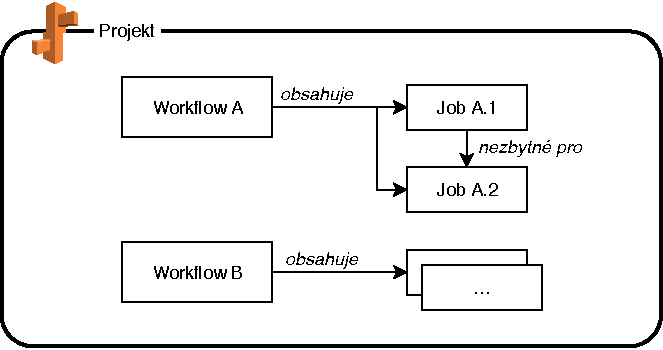
\includegraphics[width=1.0\textwidth]{media/circleci-arch.pdf}
            }
            \caption{Architektura \circleci. Každý projekt může mít několik \textit{workflows}, uvnitř které je libovolný souvislý acyklický graf \textit{jobs}.}
            \label{pic:circle-architecture}
        \end{iffigure}

        \semaphore kombinuje architekturu dvou předchozích řešení: jednotlivé joby běží ve virtuálních strojích, ale jsou provázané přes koncept bloků a data si předávají přes cache. Oproti \circleci chybí možnost zrychlit přípravu prostředí a předinstalaci závislostí Docker obrazem a přitom je na \semaphore definice pipeline výrazně složitější, než na \travis.

    \subsection{Zabezpečení}
        Ani jeden z~těchto \glstext{SaaS} \CI systémů nenabízí bug bounty. Pro \travis jsem našel jednu zprávu o~bezpečnostní chybě z~roku 2018~\cite{travis-db-drop}. Pro \circleci ani \semaphore jsem žádné zveřejněné incidenty nenašel.

    \subsection{Dostupnost}
        \circleci, \travis ani \semaphore nedefinují žádné \glstext{SLA}. Za posledních 12 měsíců měl \circleci uptime $99.90$~\%~\cite{circle-uptime}, \travis $99.93$~\%~\cite{travis-uptime}. \semaphore reportuje za poslední rok podezřele vysoký uptime $100$~\%~\cite{semaphore-uptime}.

        Kromě samotných \CI služeb jsou ale tyto služby závislé na dostupnosti úložišť kódu (GitHub, GitLab, Bitbucket, …).

    \subsection{Rozšiřitelnost}
        Pro \glstext{SaaS} řešení nelze uvažovat systémy pluginů a rozšíření. Veškerá funkcionalita služby musí být přímo integrovaná v~systému. Tyto možnosti popisuji v~následující podsekci.

    \subsection{Integrace}
        \travis lze používat pouze s~repozitáři na GitHub, \circleci a \semaphore podporují kromě toho také Bitbucket. Nelze používat vlastní repozitáře a jiné systémy. Teoreticky lze vytvořit vlastní obálku nad cizím \glstext{API} a posílat webhooky ve formátu jako GitHub, ale nejde o~oficiálně podporovanou variantu.

        \semaphore má složité zakládání nového repozitáře. Na rozdíl od ostatních dvou \CI je nutné nainstalovat na klientu spustitelný program, který podporuje pouze Linux a macOS a instaluje se přes \code{curl|bash}. Poté se v~repozitáři musí zavolat \code{sem init}, který ale funguje pouze pokud má projekt nastavený \code{origin remote} na GitHub. Běžně stačí projekt přidat v~administraci \CI: díky propojení na GitHub \CI ví, jaké projekty existují.

        Všechny tři \CI podporují GitHub perfektně a i nově zveřejněné funkce implementují rychle.

    \subsection{Praktické nasazení projektů}
        \subsubsection{Projekt 1}
            Ze všech \CI vyzkoušených v~této práci bylo nasazení na \travis suverénně nejjednodušší. Na deseti řádcích se přehledně definují všechny závislosti a volá se build. I~nezaškolený uživatel by dokázal vytvořit novou pipeline podle minimální ukázky.

            Na \circleci je konfigurace pipeline znatelně složitější. Rozdělením na kontejnery se ale separují jednotlivé závislosti a správa komplexních projektů by byla jednodušší. Další výhoda \circleci pro tento projekt je možnost opakovat pouze jenom dílčí kroky a ukládat mezivýsledky do cache, která se může použít při každém spuštění. Toho jsem využil pro instalaci závislostí z~Gemfile. Alternativou bylo vytvořit nový Docker obraz a Ruby gemy tam předinstalovat. To má ale řadu nevýhod, předně to zvyšuje komplexitu a bylo by složitější použít jiné gemy (jiná rozšíření pro Jekyll).

            Pro \semaphore jsem de facto musel zkombinovat obě předchozí řešení: v~\glstext{VM} jsem nechal nainstalovat Ruby gemy a uložil je do cache. V~druhém jobu se cache stáhne a spustí se kompilace samotného statického webu.

            Na rozdíl od ostatních nasazení jsem při testování \glstext{SaaS} neimplementovat celou \CI pipeline včetně nahrání na cílový server. Všechny systémy jsem zprovoznil v~lokálním virtuálním prostředí na které není vhodné dělat vzdálený přístup. Místo \code{make deploy} je tak v~definicích pouze job s~hláškou, kde by se deploy spouštěl.

        \subsubsection{Projekt 2}
            Pro druhý ukázkový projekt jsem upravil konfigurace vytvořené pro statickou aplikaci. Pro \circleci a \travis jsem finální funkční pipeline vytvořil na první pokus. Pro \semaphore bylo z~dokumentace nutné nastudovat, jaké obrazy pro \glstext{VM} jsou dostupné a případně jaké jsou poskytované nástroje jsou instalaci a konfiguraci závislostí. Konkrétně pro \glstext{PHP} je předinstalován nástroj phpbrew. Dále jsem musel ladit nastavení cache složky \code{vendor} ve které jsou závislosti nainstalované nástrojem \code{composer}, především aby fungovalo sdílení dat mezi krokem pro kompilaci a pro nasazení.

        \subsubsection{Projekt 3}
            Kompilace Docker obrazu byla snadná na všech třech testovaných \glstext{SaaS} \CI. Ve všech případech byla konfigurace krátká a výstižná. \travis a \semaphore, které jsou založené na virtuálních strojích, byly stejně jednoduché na konfiguraci jako \circleci, který je založený na kontejnerech a konfiguruje externí Docker daemon.
